\documentclass[a4paper]{article}
\usepackage[utf8]{inputenc}

\usepackage[a4paper, margin=1in]{geometry}
\usepackage{amsmath}

\usepackage{graphicx}
\usepackage{subcaption}

\usepackage{pdflscape}

\usepackage{listings}
\usepackage{xcolor} %for listings
\lstset{
 basicstyle=\footnotesize,
 commentstyle=\color{red},
 keywordstyle=\color{blue},
 stringstyle=\color{purple},
}

\usepackage{siunitx}

\title{Motor Controller Report}
\author{Zedd Serjeant 1261476}
\date{27 April 2020}

% \DeclareSIUnit{cycles}{cycles}


\begin{document}


\maketitle
% \setlength{\droptitle}{-10em}   % This is your set screw

\section{Device Purpose}
% The purpose of this device is to measure the depth of a water column within an acrylic tube of arbitrary diameter. This will utilise ultrasonic sonar.
The purpose of this device is to control the speed of a motor using feedback. It must be stable and stand up to system disturbance, such as friction interfering with shaft rotation.

\section{Algorithm}

\subsection{Interrupt} \label{subsect:interrupt}
There are three interrupts used to control timing. One occurs approximately every millisecond. This is used to control an LED with a duty cycle. It is set to be proportional to the potentiometer input so that the user knows what setting they have chosen.

The other two serve the purpose of controlling when the system samples the motor speed (\textit{Appendix}~\ref{sect:timing}). Each cycle, as the PWM goes low, the \textbf{Timer 2 Interrupt} is triggered. This sets another interrupt to occur after the internal inductance discharges, indicating for the mainline to measure the voltage across the motor terminals.

The discharge of the inductance is the main design factor these interrupts are based around. This system was designed around an inductance of \SI{20}{\milli\henry}, leading to a PWM rate of \SI{280}{\hertz}. A larger inductance requires a slower PWM signal, or a different approach to interrupt timing. 

\subsection{Mainline}
The body of the code is concerned with measuring the motor speed, supply voltage and the potentiometer, and using this information to calculate a duty cycle for the PWM (\textit{Appendix}~\ref{sect:timing}). This in turn sets the motor speed and the LEDs.

The Execution of the mainline is controlled by the interrupts. Each millisecond, a flag is set to measure the supply to ensure it is within the limits specified in the \textbf{Specification}(\textit{Section}~\ref{sect:specificaton}). It also uses this to make the PWM calculations more accurate, as PWM can be seen as setting a fraction of the input voltage. The design is economical for microcontroller pins, as this measurement is made with the same pin as the motor speed measurement. It does this by driving the motor, putting the full input voltage on the terminals, before the measurement.

Each full Period of the PWM, a flag is set to measure the current motor speed. This involves the delay explained in \textbf{Interrupts}(\textit{Section}~\ref{subsect:interrupt}). After this initial timed measurement, another two are made, separated by the \textit{ADC} clock speed, and a Median Filter is applied for more stability.

This process is then followed by the \textbf{Control Algorithm}(\textit{Section}~\ref{subsect:control_method}).

The final task of the Mainline then immediately follows this: The potentiometer is read, and the result interpreted as a voltage to set the motor speed to, a value ranging between \SI{1.47}{\volt} to \SI{8}{\volt}. This range was chosen empirically and to meet the specification. At \SI{1.47}{\volt}, the motor cannot be reliably run without control, and a voltage above \SI{8}{\volt} cannot be guaranteed within the specification, so no attempt to support this can be made.


\subsection{Control Method} \label{subsect:control_method}
This controller implements \textbf{PI} control.

Each cycle of PWM, the output drops low, triggering an interrupt. The system waits a certain amount of time (\SI{34}{\micro\second}) to allow the \textit{motor inductance} to discharge. Three measurements are made and the median taken to give $\mathbf{V_M}$, the voltage of the motor which is representative of shaft speed.

The error is calculated as in \textit{Equation}~\ref{eq:error_equation} and is numerically integrated (summed) over time as \textit{Equation}~\ref{eq:error_sum_equation}

\begin{equation} \label{eq:error_equation}
    \text{error} = \text{set point} - V_M 
\end{equation}

\begin{equation} \label{eq:error_sum_equation}
    \text{error sum} = \int_0^t \textbf{error}\,\mathrm{d}t = \sum_{i=0}^t \textbf{error}(t) 
    \implies \textit{error sum += error}
\end{equation}

These values are used in a feedback loop to set the speed as in \textit{Equation}~\ref{eq:pi_calculation}, where the values of $k_p$ and $k_i$ are set to lead to a stable and fast response.  

\begin{equation} \label{eq:pi_calculation}
    \text{output} = (\text{set point}) + k_p\cdot(\text{error}) + k_i\cdot(\text{error sum})
\end{equation}



\section{Hardware Design}
The hardware was built with one major constraint: Only components that could be quickly gathered before the initiation of lock down could be used. This limited the resistor and capacitor values that were available, along with forcing the use of a P-type FET. 

The circuit sections with interesting design choices are:
\begin{itemize}
    \item The Programming Header
    \item The voltage regulator and associated bypass capacitors
    \item The Feedback voltage divider
    \item Motor Control
\end{itemize}

The programming header was implemented to enable \textit{In Circuit Serial Programming}(\textbf{ICSP}). This is beneficial as it allows faster prototyping and then fast manufacture.

The voltage regulator is necessary to allow the PIC to function under the fluctuating high range input. This input also has a large level of noise due to the motor being directly connected to this source. Thus Bypass capacitors are necessary, and their values are chosen based on recommended values from the regulators datasheet, and drawn from the limited pool.

To sense the speed of the motor, the voltage across its terminals needs to be read by the ADC. As this voltage can be up to \SI{16}{\volt} per the specification, a resistive divider is employed to scale this voltage down to a maximum of \SI{5}{\volt}. The first resistor was chosen to be \SI{10}{\kilo\ohm} to limit current though this branch, while the second was chosen to meet the ratio of $5/16$.

The Motor, as mentioned is driven by a P-FET rather than the traditional N-FET in a bootstrap configuration. While this made the design simpler it also made the circuit more inefficient. The FET is driven by a BJT controlling the presence of the supply voltage on the gate, allowing the small voltages of the microcontroller to control the motor.

%  Brief description of what the components in the circuit do, a “how it works”, indicating how
% critical component values were chosen, what groups of components achieve, etc.



\section{Testing and Operating}
Whilst the system is running the circuit provides features for user feedback and user adjustment.

There are three LED, one that indicates the current value of the potentiometer as a ratio of duty cycle to period, another that glows when the control loop is offset from the set point by too large a value (currently \SI{1.5}{\volt}) and the final LED glows when the circuit is in an error state. The system indicates an error when the supply voltage is outside of specification. 

A user knows the system is running well when they can set a motor speed using the POT, causing the POT LED to change, and then the loop-offset LED settles into being off the majority of the time. If the system ever malfunctions, either the loop-offset LED or the error LED will be on permanently. If this is a software error, there is a button attached to induce a soft-reset; pressing the button sets all internal error values to zero and temporarily disables the control loop until the system stabilises.

If the user notices some instability in the control loop, there is a process by which they can adjust the internal control constants:
\begin{enumerate}
    \item set the motor speed to zero via the potentiometer
    \item Press the button. Instead of initiating a reset, this will now adjust the system mode
    \item The first mode adjusts the proportion constant. The motor will vary up and down across is full speed range, while the potentiometer now sets the proportion constant
    \item Any press of the button will save the new proportion constant, and move the system into integral-constant-set-mode. The motor will continue to vary and the potentiometer will now set the integral constant.
    \item Any press of the button will now save the current integral value and move back to proportion set mode
    \item To return to speed control, cycle the power.
\end{enumerate}

When these circuits go through manufacture, these features can be used to ensure the product is ready for release.

The circuit is powered and placed into constant set mode. As the motor speed varies, the loop-offset LED is observed (either by a manufacture system or a human). If the system is not responding well enough, the constants can be adjusted until it is.

%  What indications your circuit provides that it is operating successfully.
 
%   Description of an electronic test that will demonstrate that the feedback is operating, as a
% sort of “manufacturing check” that can be applied to a circuit once built.



\newpage
\section{Appendix - Specification} \label{sect:specificaton}
Here are the specifications as laid out by the \textit{Project Manager} 
\begin{itemize}
    \item Goal: keep the rotational speed of the motor shaft constant, as set by the Input Potentiometer.
    
    \item Both the code and circuit need to be designed in tandem, with LEDs serving as outputs of useful information.
    
    \item The system is required to run on a variable supply of \SI{8}{\volt} to \SI{16}{\volt}.
    
    \item The Control loop may not oscillate around the set point excessively.
\end{itemize} 


\newpage
\section{Appendix - Timing} \label{sect:timing}
Various Figures showing the timing of different important parts of the program

\begin{figure}[h!]
    \centering
    \includegraphics[width=0.5\textwidth]{img/InterruptTiming.png}
    \caption{Interrupt Time - high when within the interrupt}
\end{figure}

\begin{figure}[h!]
    \centering
    \includegraphics[width=0.5\textwidth]{img/mainline.png}
    \caption{Mainline PWM generation - Orange:Motor, Blue:PWM, Green:Potentiometer}
\end{figure}

\begin{figure}[h!]
    \centering
    \includegraphics[width=0.5\textwidth]{img/sampling.png}
    \caption{Sampling - Orange: Motor, Blue: PWM, Green: Potentiometer, Purple: Sampling Interrupt}
\end{figure}



\newpage
\pagestyle{empty}
\newgeometry{margin=1cm}
\begin{landscape}

\section{Appendix - Software}
%XXX - reformat, change margins, add colour coding
\subsection{head.h}
\lstinputlisting[language=C]{../../MotorController.X/head.h}
\newpage
\subsection{main.c}
\lstinputlisting[language=C]{../../MotorController.X/main.c}

\newpage
\section{Appendix - Hardware} \label{sect_hardware}

\begin{figure}[b!]
    \centering
    \includegraphics[width=1.3\textwidth]{img/hardware_schematic.PNG}
    \caption{Hardware Schematic}
    \label{fig:hardware_schematic}
\end{figure}

\begin{figure}[b!]
    \centering
    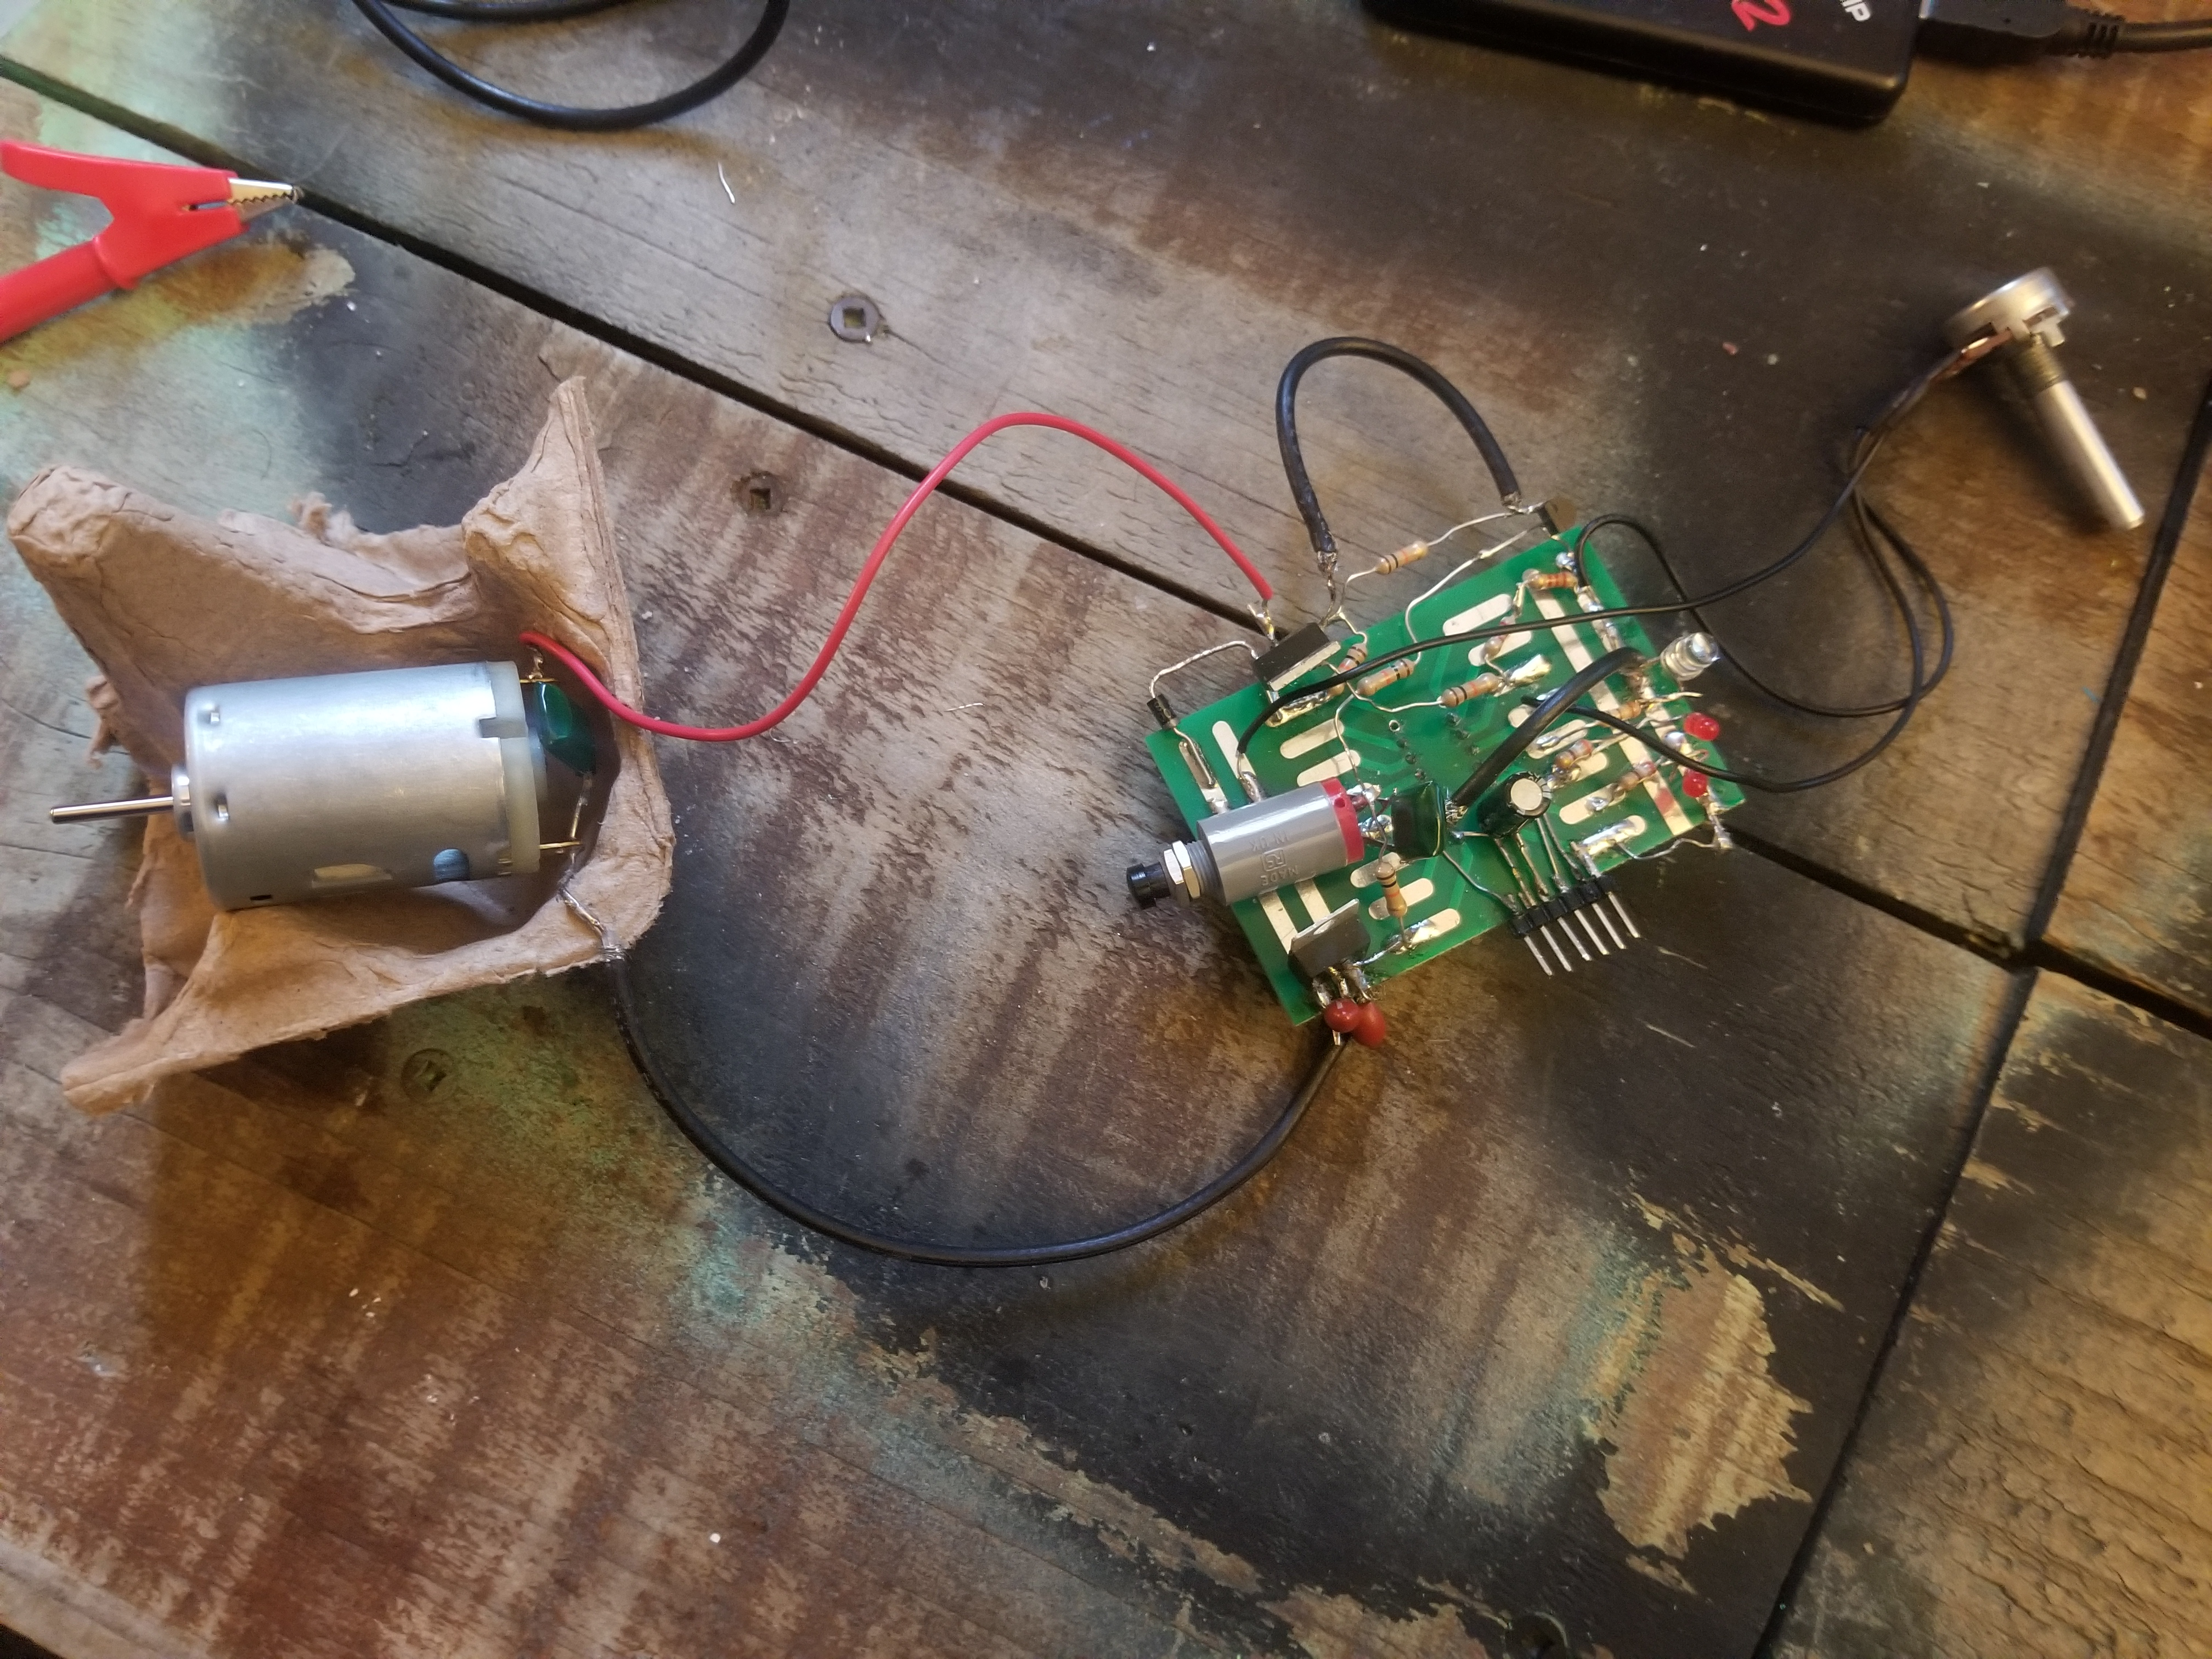
\includegraphics[width=\textwidth]{img/system_prototype.PNG}
    \caption{Hardware Prototype Top-down}
    \label{fig:system}
\end{figure}

\begin{figure}[b!]
    \centering
    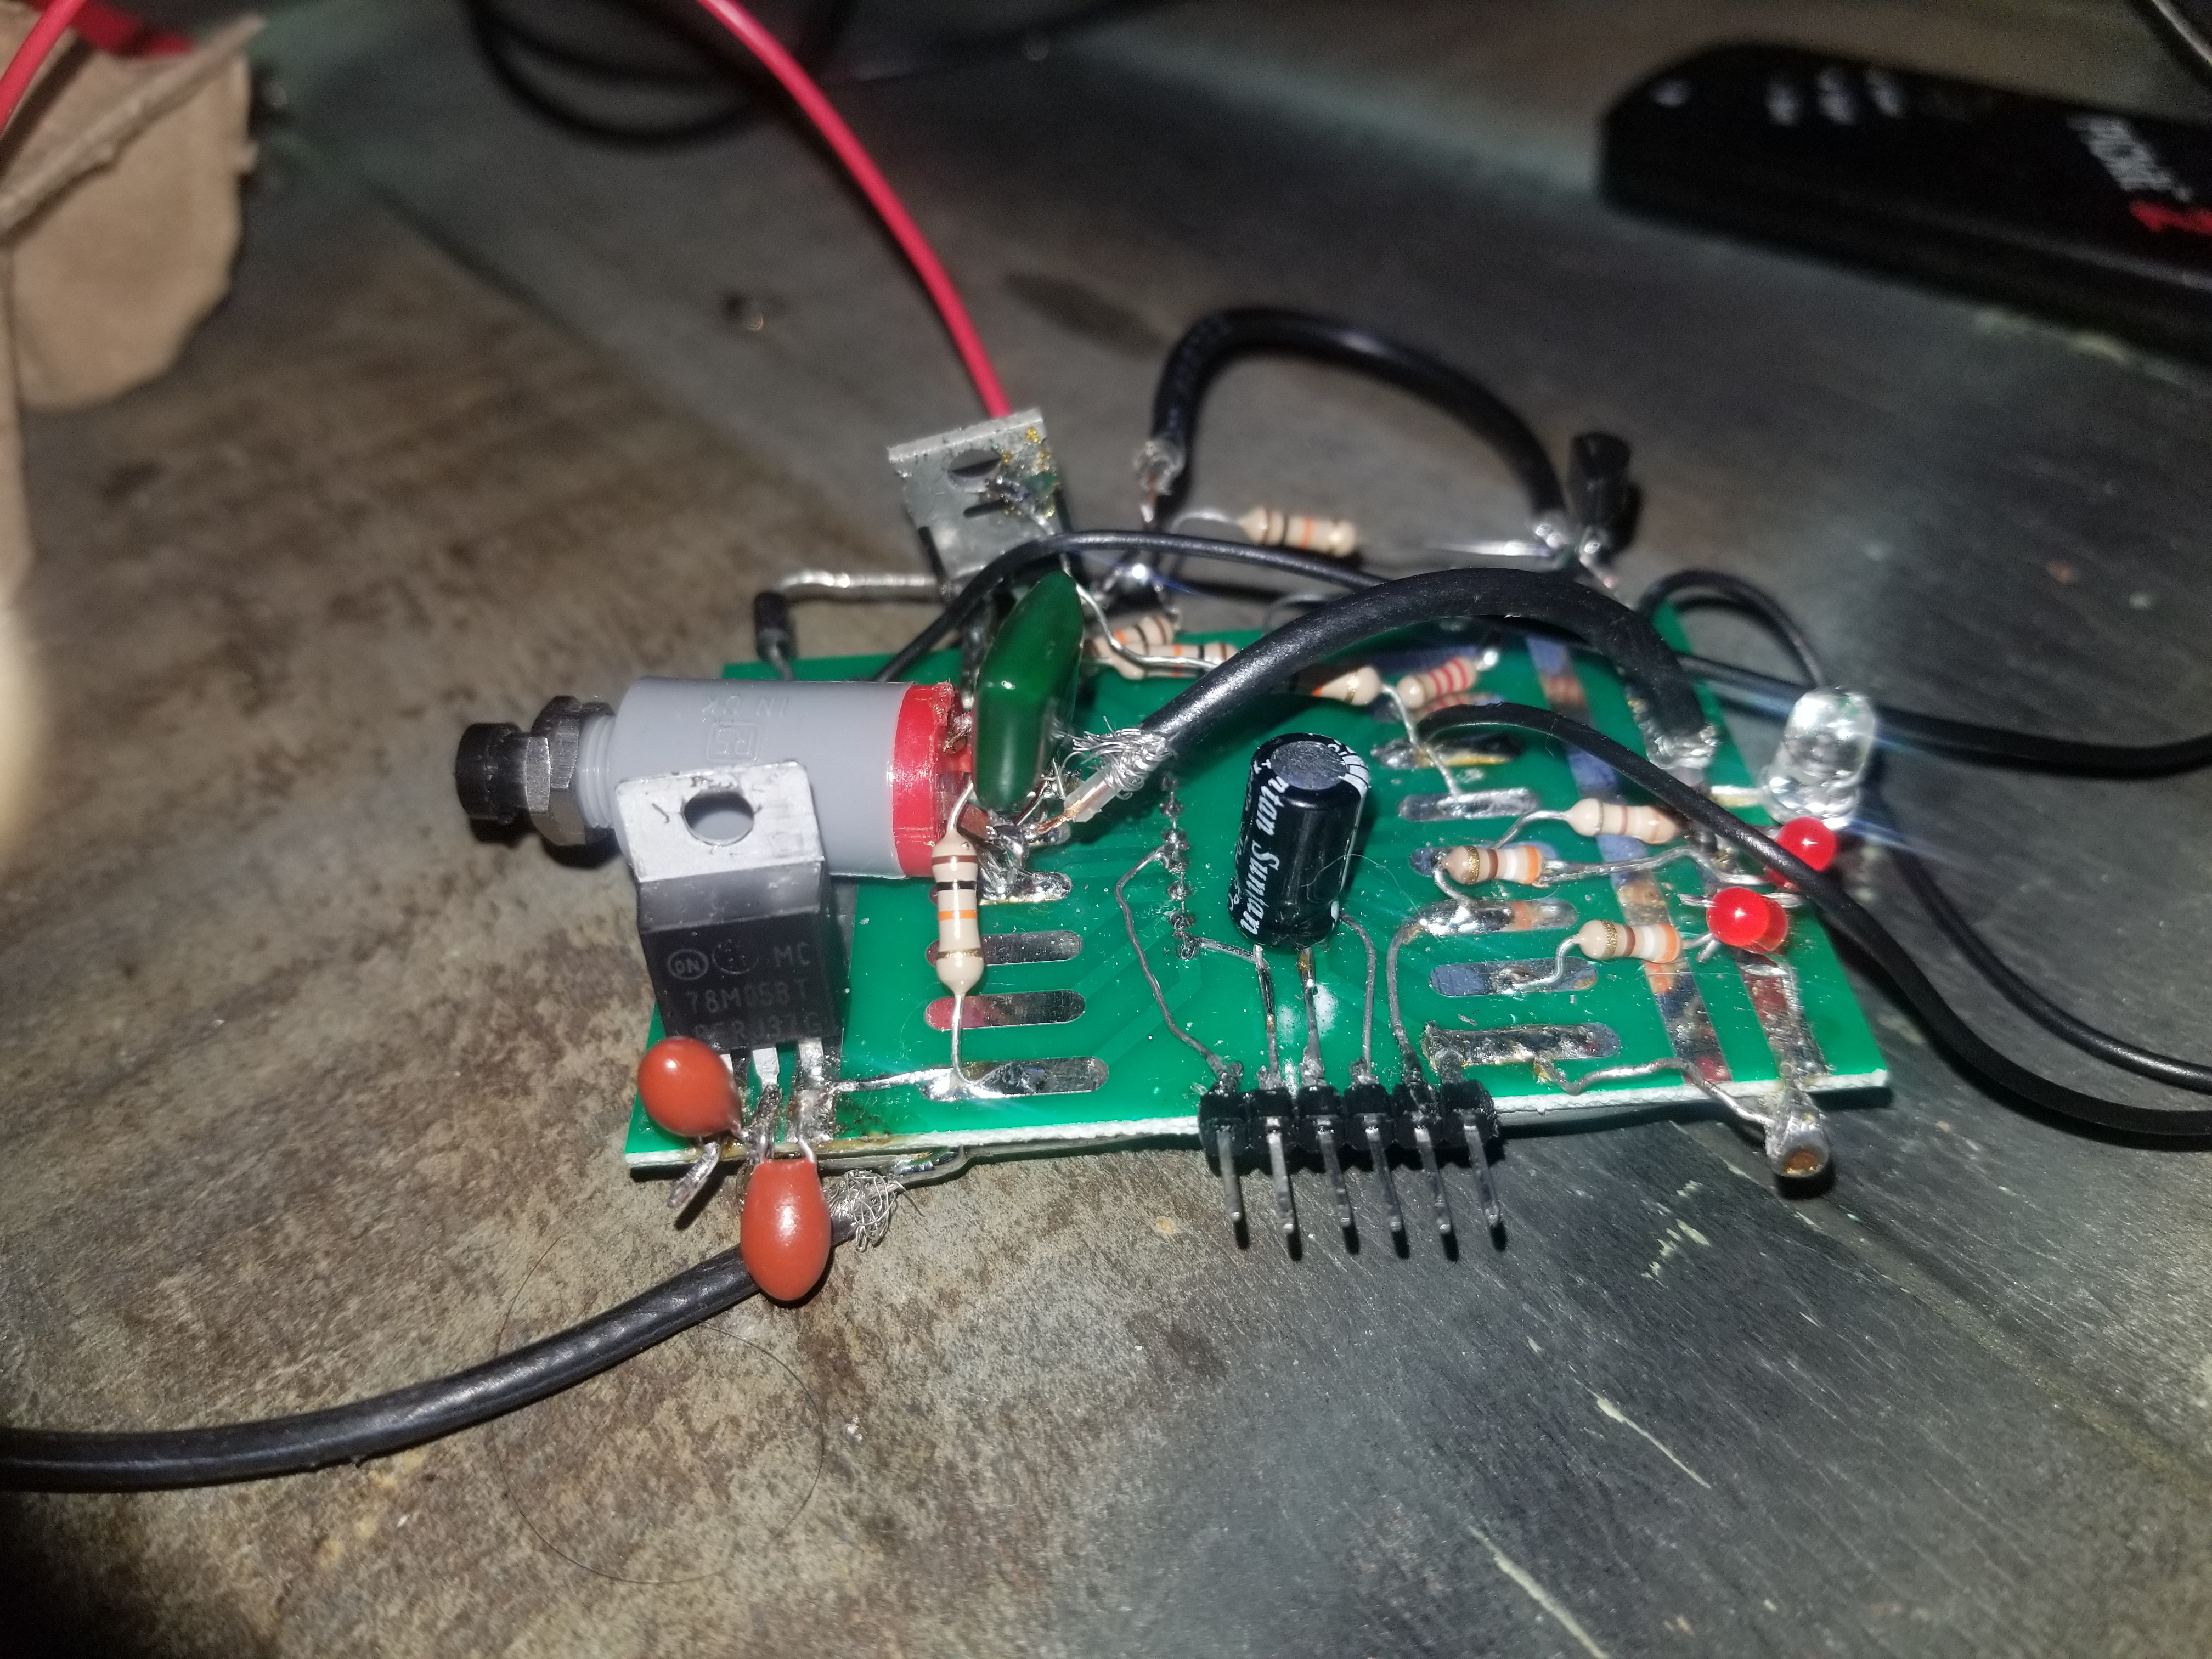
\includegraphics[width=\textwidth]{img/circuitboard_prototype.png}
    \caption{Hardware Prototype Circuit Board}
    \label{fig:circuitboard}
\end{figure}

\end{landscape}
\end{document}
